\section{Cells}

Let us first introduce a discrete version of the familiar 2-dimensional Euclidean space. Two-dimensional space supports objects with either zero, one, or two dimensions, such as points, lines, and planes. These $k$-dimensional objects are named $k$-cells, represented by $\sigma^{(k)}$, where $k$ denotes the dimension of the cell. Three examples of $k$-cells are shown in Figure \ref{fig:cells}.
\begin{figure}[ht]
    \newsavebox\boxCell
    \savebox{\boxCell}{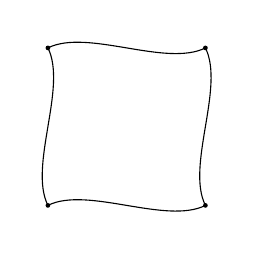
\begin{tikzpicture}
        \fill (0,0) circle (0.03);
        \fill (2,0) circle (0.03);
        \fill (2,2) circle (0.03);
        \fill (0,2) circle (0.03);
        \draw (0,0) .. controls (0.5,0.25) and (1.5,-0.25) .. (2,0) .. controls (1.75,0.5) and (2.25,1.5) .. (2,2) .. controls (1.5,1.75) and (0.5,2.25) .. (0,2) .. controls (0.25,1.5) and (-0.25,0.5) .. (0,0);
    \end{tikzpicture}}
    \centering
    \begin{subfigure}[c]{0.3\textwidth}
        \centering
        \vbox to \ht\boxCell{
            \vfill
            \begin{tikzpicture}
                \fill (1,1) circle (0.03);
            \end{tikzpicture}
            \vfill
        }
        \caption{0-cell}
    \end{subfigure}
    \begin{subfigure}[c]{0.3\textwidth}
        \centering
        \vbox to \ht\boxCell{
            \vfill
            \begin{tikzpicture}
                \fill (0,1) circle (0.03);
                \draw (0,1) .. controls (0.5,1.25) and (1.5,0.75) .. (2,1);
                \fill (2,1) circle (0.03);
            \end{tikzpicture}
            \vfill
        }
        \caption{1-cell}
    \end{subfigure}
    \begin{subfigure}[c]{0.3\textwidth}
        \centering
        \usebox{\boxCell}
        \caption{2-cell}
        \label{fig:2cell}
    \end{subfigure}
    \caption{Examples of $k$-cells in two-dimensional space.}
    \label{fig:cells}
\end{figure}

A point or scalar is a 0-cell and a line segment or vector is a 1-cell. Just like a 1-cell is a line with a length but with no position, a 2-cell can be thought of as a plane with an area, but no position.

Notice that $k$-cells are bounded by $(k-1)$-cells and that a cell's shape is arbitrary, as indicated by the wavy lines in Figure \ref{fig:cells}. (\textit{Note:} The boundary of 0-cells is empty by definition.) A set of $k$-cells is called a cell-complex iff the boundary of each $k$-cell is also part of the set. For example, the object in Figure \ref{fig:2cell} is a cell-complex because the plane is bounded by lines and the lines are in turn bounded by points, all of which are part of the object.

\section{Chains and Cochains}

A set of $k$-cells is called a chain, written as
\begin{equation}
    \mathbf{c}^{(k)} = \{c_1 \sigma^{(k)}_1, \ldots, c_N \sigma^{(k)}_N \}
\end{equation}
where $N$ denotes the number of $k$-cells in the cell complex and $c_i$ denotes a weight $\in \mathbb{R}$. Chains merely differ by their weights, since all chains are composed of the same $k$-cells. The summation and multiplication of two $k$-chains is well-defined. In the case of summation, the weights add, and in the case of multiplication by a real number, the weights are multiplied by that real number. Thus, the set of $k$-chains, denoted $C^{(k)}$, is a linear vector space and the $k$-cells represent a basis for this vector space.

Because $k$-cells represent a basis for $C^{(k)}$, we can define linear functionals that assign a value to $k$-cells. These linear functionals are called $k$-cochains and the set of all $k$-cochains is itself a linear vector space. To reiterate the main point: a chain is a set of cells and a cochain is a linear map from a set of cells to a set of numbers.

\section{Orientation}

In addition to their dimension, $k$-cells have a property that we call orientation. A $k$-cell either has a positive or a negative orientation that can be freely defined on a per-cell basis, as long as the orientation remains unchanged thereafter. 

Figure \ref{fig:innerExample} shows three $k$-cells in two-dimensional space with an intrinsic orientation that we call inner-oriented $k$-cells. Inner-oriented points for instance, can either represent sources or sinks and are arbitrarily chosen to be sources (i.e. positive) by default, as indicated by the outward pointing arrows in Figure \ref{fig:inner0Cell}. Inner-oriented lines have a positive orientation when pointing to the right, as indicated by the arrows in Figure \ref{fig:inner1Cell}. It is a bit awkward to think of the orientation of a plane, but an inner-oriented plane is defined positive when it is oriented counterclockwise, as indicated in Figure \ref{fig:inner2Cell}.

Inner-oriented $k$-cells have an outer-oriented counterpart where its orientation is defined around or through the $k$-cell, rather than within. For example, an inner-oriented surface has a counterclockwise orientation whereas an outer-oriented surface represents a source. Figure \ref{fig:outerExample} shows three outer-oriented $k$-cells in two-dimensional space.
\begin{figure}[ht]
    \newsavebox\boxInner
    \savebox{\boxInner}{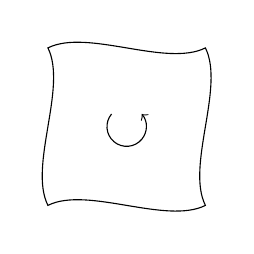
\begin{tikzpicture}
        \draw (0,0) .. controls (0.5,0.25) and (1.5,-0.25) .. (2,0) .. controls (1.75,0.5) and (2.25,1.5) .. (2,2) .. controls (1.5,1.75) and (0.5,2.25) .. (0,2) .. controls (0.25,1.5) and (-0.25,0.5) .. (0,0) -- cycle;
        \draw [->] (1,1) ++(140:0.25) arc (-220:40:0.25);
    \end{tikzpicture}}
    \centering
    \begin{subfigure}[c]{0.3\textwidth}
        \centering
        \vbox to \ht\boxInner{
            \vfill
            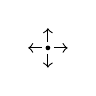
\begin{tikzpicture}
                \fill (1,1) circle (0.03);
                \draw [->] (1,1.075) -- (1,1.25);
                \draw [->] (1.075,1) -- (1.25,1);
                \draw [->] (1,0.925) -- (1,0.75);
                \draw [->] (0.925,1) -- (0.75,1);
            \end{tikzpicture}
            \vfill
        }
        \caption{0-cell}
        \label{fig:inner0Cell}
    \end{subfigure}
    \begin{subfigure}[c]{0.3\textwidth}
        \centering
        \vbox to \ht\boxInner{
            \vfill
            \begin{tikzpicture}
                \draw (0,1) .. controls (0.5,1.25) and (1.5,0.75) .. (2,1);
                \draw [->] (0.95,1.008) -- (1.05,0.992);
            \end{tikzpicture}
            \vfill
        }
        \caption{1-cell}
        \label{fig:inner1Cell}
    \end{subfigure}
    \begin{subfigure}[c]{0.3\textwidth}
        \centering
        \centering
        \usebox{\boxInner}
        \caption{2-cell}
        \label{fig:inner2Cell}
    \end{subfigure}
    \caption{Inner-oriented $k$-cells in two-dimensional space.}
    \label{fig:innerExample}
\end{figure}
\begin{figure}[ht]
    \newsavebox\outerBox
    \savebox{\outerBox}{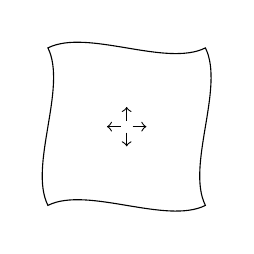
\begin{tikzpicture}
        \draw (0,0) .. controls (0.5,0.25) and (1.5,-0.25) .. (2,0) .. controls (1.75,0.5) and (2.25,1.5) .. (2,2) .. controls (1.5,1.75) and (0.5,2.25) .. (0,2) .. controls (0.25,1.5) and (-0.25,0.5) .. (0,0) -- cycle;
        \draw [->] (1,1.075) -- (1,1.25);
        \draw [->] (1.075,1) -- (1.25,1);
        \draw [->] (1,0.925) -- (1,0.75);
        \draw [->] (0.925,1) -- (0.75,1);
    \end{tikzpicture}}
    \centering
    \begin{subfigure}[c]{0.3\textwidth}
        \centering
        \vbox to \ht\outerBox{
            \vfill
            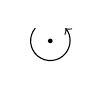
\begin{tikzpicture}
                \fill (1,1) circle (0.03);
                \draw [->] (1,1) ++(140:0.25) arc (-220:40:0.25);
            \end{tikzpicture}
            \vfill
        }
        \caption{0-cell}
    \end{subfigure}
    \begin{subfigure}[c]{0.3\textwidth}
        \centering
        \vbox to \ht\outerBox{
            \vfill
            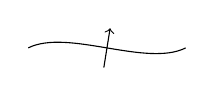
\begin{tikzpicture}
                \draw (0,1) .. controls (0.5,1.25) and (1.5,0.75) .. (2,1);
                \draw [->] (0.96,0.75) -- (1.04,1.25);
            \end{tikzpicture}
            \vfill
        }
        \caption{1-cell}
    \end{subfigure}
    \begin{subfigure}[c]{0.3\textwidth}
        \centering
        \usebox{\outerBox}
        \caption{2-cell}
    \end{subfigure}
    \caption{Outer-oriented $k$-cells in two-dimensional space.}
    \label{fig:outerExample}
\end{figure}

The distinction between inner and outer oriented $k$-cells makes sense from a physical point of view; certain physical quantities are naturally expressed in terms of inner-oriented cochains whereas other physical quantities are naturally expressed in terms of outer-oriented cochains. The circulation along a line naturally resembles an inner-oriented 1-cell whereas the flux through a line naturally resembles an outer-oriented 1-cell.

\section{The Exterior Derivative}

The descrete exterior derivative, $\delta$, is a linear map of a $(k)$-cochain to a $(k+1)$-cochain. It turns out that the standard treatment of vector calculus hides a number of important things that are applied implicitly. As we shall see in the upcoming examples, all three of the multivariable derivatives in vector calculus (i.e. gradient, curl, and divergence) are actually one kind of derivative: the exterior derivative.

\subsection{Inner-Oriented Quantities}

\begin{figure}[ht]
    \newsavebox\boxExample
    \savebox{\boxExample}{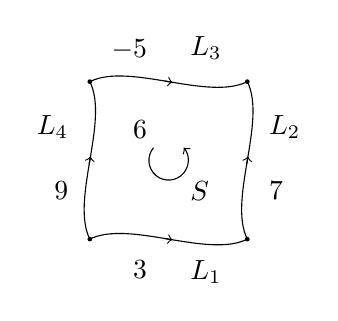
\begin{tikzpicture}
        \fill (0,0) circle (0.03) node [below left=1ex] at (1,0) {3} node [below right=1ex] at (1,0) {$L_1$};
        \fill (2,0) circle (0.03) node [below right=1ex] at (2,1) {7} node [above right=1ex] at (2,1) {$L_2$};
        \fill (2,2) circle (0.03) node [above left=1ex] at (1,2) {$-5$} node [above right=1ex] at (1,2) {$L_3$};
        \fill (0,2) circle (0.03) node [below left=1ex] at (0,1) {9} node [above left=1ex] at (0,1) {$L_4$};
        \draw (0,0) .. controls (0.5,0.25) and (1.5,-0.25) .. (2,0) .. controls (1.75,0.5) and (2.25,1.5) .. (2,2) .. controls (1.5,1.75) and (0.5,2.25) .. (0,2) .. controls (0.25,1.5) and (-0.25,0.5) .. (0,0) -- cycle;
        \draw [->] (1,1) ++(140:0.25) arc (-220:40:0.25) node [above left=1ex] at (1,1) {6} node [below right=1ex] at (1,1) {$S$};
        \draw [->] (0.95,0.008) -- (1.05,-0.008);
        \draw [->] (1.992,0.95) -- (2.008,1.05);
        \draw [->] (0.95,2.008) -- (1.05,1.992);
        \draw [->] (-0.008,0.95) -- (0.008,1.05);
    \end{tikzpicture}}
    \centering
    \begin{subfigure}[c]{0.3\textwidth}
        \centering
        \vbox to \ht\boxExample{
            \vfill
            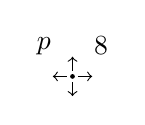
\begin{tikzpicture}
                \fill (1,1) circle (0.03) node [above right=1ex] {8} node [above left=1ex] {$p$};
                \draw [->] (1,1.075) -- (1,1.25);
                \draw [->] (1.075,1) -- (1.25,1);
                \draw [->] (1,0.925) -- (1,0.75);
                \draw [->] (0.925,1) -- (0.75,1);
            \end{tikzpicture}
            \vfill
        }
        \caption{0-cochain}
        \label{fig:0cochainExample}
    \end{subfigure}
    \begin{subfigure}[c]{0.3\textwidth}
        \centering
        \vbox to \ht\boxExample{
            \vfill
            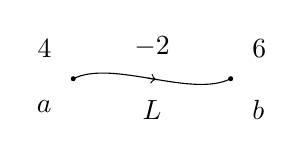
\begin{tikzpicture}
                \fill (0,1) circle (0.03) node [above left=1ex] {4};
                \fill (0,1) circle (0.03) node [below left=1ex] {$a$};
                \draw (0,1) .. controls (0.5,1.25) and (1.5,0.75) .. (2,1);
                \fill (2,1) circle (0.03) node [above right=1ex] {6};
                \fill (2,1) circle (0.03) node [below right=1ex] {$b$};
                \draw [->] (0.95,1.008) -- (1.05,0.992) node [above=1ex] at (1,1) {$-2$} node [below=1ex] at (1,1) {$L$};
            \end{tikzpicture}
            \vfill
        }
        \caption{1-cochain}
        \label{fig:1cochainExample}
    \end{subfigure}
    \begin{subfigure}[c]{0.3\textwidth}
        \centering
        \usebox{\boxExample}
        \caption{2-cochain}
        \label{fig:2cochainExample}
    \end{subfigure}
    \caption{Examples of $k$-cochains in two-dimensional space.}
    \label{fig:cochainExamples}
\end{figure}

Figure \ref{fig:1cochainExample} shows a 0-cochain consisting of two points, $a$ and $b$, and a 1-cochain consisting of one line segment, $L$. $L$ points from $a$ to $b$, so $a$ acts as a source and $b$ acts as a sink. Because a sink is defined negative, application of $\delta$ results in a value of $-2$ assigned to the line segment, since $4 - 6 = -2$. Assuming that points represent samples of a continuous scalar field, $\phi$, it is clearly seen that the application of $\delta$ on a 0-cochain is analogous to the gradient operator:
\begin{equation}
    \begin{split}
        4 - 6 &= \phi(b) - \phi(a) \\
        &= \int_{L} \nabla \phi \cdot d\mathbf{s}
    \end{split}
\end{equation}

Figure \ref{fig:2cochainExample} shows a 1-cochain consisting of four line segments and a 2-cochain consisting of a surface, $S$. If the orientation of a boundary line segment opposes the orientation of the surface, then its value should be subtracted. Thus, application of $\delta$ results in a value of $6$ assigned to the surface, since $3 - 7 - (-5) - 9 = 6$. If line segments represent paths through a vector field, $\mathbf{u}$, then the application of $\delta$ on a 1-cochain is analogous to the curl operator:
\begin{equation}
    \begin{split}
        4 + 7 - (-8) - 9 &= \int_{L_1} \mathbf{u} \cdot \mathbf{dl} + \int_{L_2} \mathbf{u} \cdot \mathbf{dl} + \int_{L_3} \mathbf{u} \cdot \mathbf{dl} + \int_{L_4} \mathbf{u} \cdot \mathbf{dl} \\
        &= \oint_{\partial S} \mathbf{u} \cdot \mathbf{dl} \\
        &= \iint_{S} \left( \nabla \times \mathbf{u} \right) \cdot dA
    \end{split}
    \label{eq:curlExample}
\end{equation}
where $\partial S \equiv L_1 \cup L_2 \cup L_3 \cup L_4$. This is not the only insight to be gained here. Suppose that the vector field $\mathbf{u}$ represents a velocity field. Recall that the circulation, denoted $\Gamma$, is defined as:
\begin{equation}
    \Gamma \equiv \oint_C \mathbf{u} \cdot \mathbf{dl}
    \label{eq:circulation}
\end{equation}
Comparing Equations \eqref{eq:curlExample} and \eqref{eq:circulation}, we conclude that if a line segment represents a velocity vector, then a surface must represent the circulation around its boundary. Circulation is related to vorticity; the circulation around a closed contour is equal to the integrated vorticity enclosed by that contour. From Stokes' theorem:
\begin{equation}
    \Gamma \equiv \oint_C \mathbf{u} \cdot \mathbf{dl} = \iint_A \left( \nabla \times \mathbf{u} \right) dA = \iint_A \xi dA
\end{equation}
Therefore, if the area of $S$ is infinitesimal, then $S$ physically represents vorticity.

Because $3$-cochains are undefined in two-dimensional space, the application of $\delta$ on a 2-cochain results in the empty set by definition. In a similar vein, 0-cochains can only be the result of the application of $\delta$ on a real number. The results of this section can be summarized in a diagram called the DeRham complex:
\begin{equation}
    \begin{gathered}
        \xymatrix@C=13ex{
            \mathbb{R} \ar[r]^{\delta} & C^{(0)} \ar[r]^{\delta}_{\text{grad}} & C^{(1)} \ar[r]^{\delta}_{\text{curl}} & C^{(2)} \ar[r]^{\delta} & \emptyset
        }
    \end{gathered}
\end{equation}

\subsection{Outer-Oriented Quantities}

The analogy between the $\delta$ operator and the gradient and curl operator applies to both inner and outer oriented $k$-cochains. Thus, the DeRham complex can be extended to include outer-oriented cochains, marked with a tilde:
\begin{equation}
    \begin{gathered}
        \xymatrix@C=13ex{
            \mathbb{R} \ar[r]^{\delta} & \tilde{C}^{(0)} \ar[r]^{\delta}_{\text{grad}} & \tilde{C}^{(1)} \ar[r]^{\delta}_{\text{curl}} & \tilde{C}^{(2)} \ar[r]^{\delta} & \emptyset
        }
    \end{gathered}
\end{equation}

\section{The Hodge-$\star$ Operator}

We have established that two-dimensional space supports points, lines, and planes. Let us briefly digress to three-dimensional space for the sake of familiarity; three-dimensional space supports points, lines, planes, and volumes. In three-dimensional space, we can have one linearly independent volume, three linearly independent planes, and three linearly independent lines. It is a bit awkward to think of linearly independent points, but there is just one linearly independent point in three-dimensional space. This 1--3--3--1 sequence suggests a pairing; there exists a vector space isomorphism between $k$-vectors and $(n-k)$-vectors. The Hodge-$\star$ operator is a linear map between inner-oriented $k$-cochains and outer-oriented $(n-k)$-cochains or vice versa, where $n$ denotes the dimension of the vector space.

We have introduced the $\delta$ operator to map $(k)$-cochains to $(k+1)$-cochains. However, the Navier-Stokes equations equate both inner and outer oriented cochains, which requires the Hodge-$\star$ operator. The Hodge-$\star$ operator links the DeRham complexes for inner and outer oriented cochains. This linked structure is called the double DeRham complex:
\begin{equation}
    \begin{gathered}
        \xymatrix@=13ex{
            \mathbb{R} \ar[r]^{\delta} & C^{(0)} \ar[r]^{\delta}_{\text{grad}} \ar@{<->}[d]^{\star} & C^{(1)} \ar[r]^{\delta}_{\text{curl}} \ar@{<->}[d]^{\star} & C^{(2)} \ar@{<->}[d]^{\star} \ar[r]^{\delta} & \emptyset \\
            \emptyset & \tilde{C}^{(2)} \ar[l]_{\delta} & \tilde{C}^{(1)} \ar[l]_{\delta}^{\text{curl}} & \tilde{C}^{(0)} \ar[l]_{\delta}^{\text{grad}} & \mathbb{R} \ar[l]_{\delta}
        }
    \end{gathered}
    \label{eq:doubleDeRham}
\end{equation}

In a discrete setting, cochains are stored in vectors, $\delta$ operators are represented by incidence matrices, $\mathbb{E}$, and Hodge-$\star$ operators are represented by Hodge matrices, $\mathbb{H}$. In such a framework, application of the $\delta$ or Hodge-$\star$ operator becomes a matrix vector-multiplication. Hence, the double DeRham complex in Equation \eqref{eq:doubleDeRham} becomes
\begin{equation}
    \begin{gathered}
        \xymatrix@=13ex{
            C^{(0)} \ar[r]^{\mathbb{E}^{(1,0)}}_{\text{grad}} \ar@<1ex>[d]^{\mathbb{H}^{(\tilde{2},0)}} & C^{(1)} \ar[r]^{\mathbb{E}^{(2,1)}}_{\text{curl}} \ar@<1ex>[d]^{\mathbb{H}^{(\tilde{1},1)}} & C^{(2)} \ar@<1ex>[d]^{\mathbb{H}^{(\tilde{0},2)}} \\
            \tilde{C}^{(2)} \ar@<1ex>[u]^{\mathbb{H}^{(0,\tilde{2})}} & \tilde{C}^{(1)} \ar[l]_{\tilde{\mathbb{E}}^{(2, 1)}}^{\text{curl}} \ar@<1ex>[u]^{\mathbb{H}^{(1,\tilde{1})}} & \tilde{C}^{(0)} \ar[l]_{\tilde{\mathbb{E}}^{(1,0)}}^{\text{grad}} \ar@<1ex>[u]^{\mathbb{H}^{(2,\tilde{0})}}
        }
    \end{gathered}
\end{equation}
